\chapter{Testy i weryfikacja jakości oprogramowania}
\label{Chapter7}

\section{Wstęp}
\label{Chapter71}

Testy i weryfikacja jakości oprogramowania realizowana była na~trzech poziomach: testów jednostkowych (dla~logiki) oraz automatycznych i~manualnych testów akceptacyjnych. Te~ostatnie realizowane były nie~tylko w~zgodzie z~dokumentem \textit{MAT}\footnote{\cite{Redmine:ProjDocs}}, ale~też intuicyjnie, poprzez normalne korzystanie z~systemu.

\section{Testy jednostkowe}
\label{Chapter72}

Testy jednostkowe zostały wykonane jako pierwsze i~traktowane były z~wysokim priorytetem. Realizowane były z~użyciem klas \textit{PHPUnit}, stosowanych powszechnie m.in.~przy testowaniu wtyczek do~platformy \textit{Moodle}. Testy~te~były kluczowe dla~rozwoju logiki systemu iQuest. Przygotowane zostały też~konfigurowalne skrypty automatyzujące proces testowania w~języku \textit{BASH}. Część testów operuje na~systemie w~trybie produkcyjnym, część~na~trybie testowym, obsługującym tzw.~,,atrapy'' (ang.~\definicja{mock}), imitujące działanie systemów zewnętrznych poprzez zwracanie przykładowych danych.\\

Przy realizacji pierwszego wydania, za~testy jednostkowe w~pełni odpowiadał jeden z~członków zespołu programistów. W wydaniu drugim, rolę~tę przejął programista realizujący logikę systemu. Planowano stosować technikę \textit{Test-Driven Development}~(TDU) - rozwój w~oparciu o~testy), jednakże szybko zrezygnowano z~tego pomysłu. Przyczyną był brak doświadczenia programistów w~tej materii. Więcej informacji o~problemach i~rozwiązaniach przyjętych przy~wykonywaniu testów znaleźć można w~rozdziale \ref{Chapter62b}.

\newpage
\begin{figure}[H]
\begin{center}
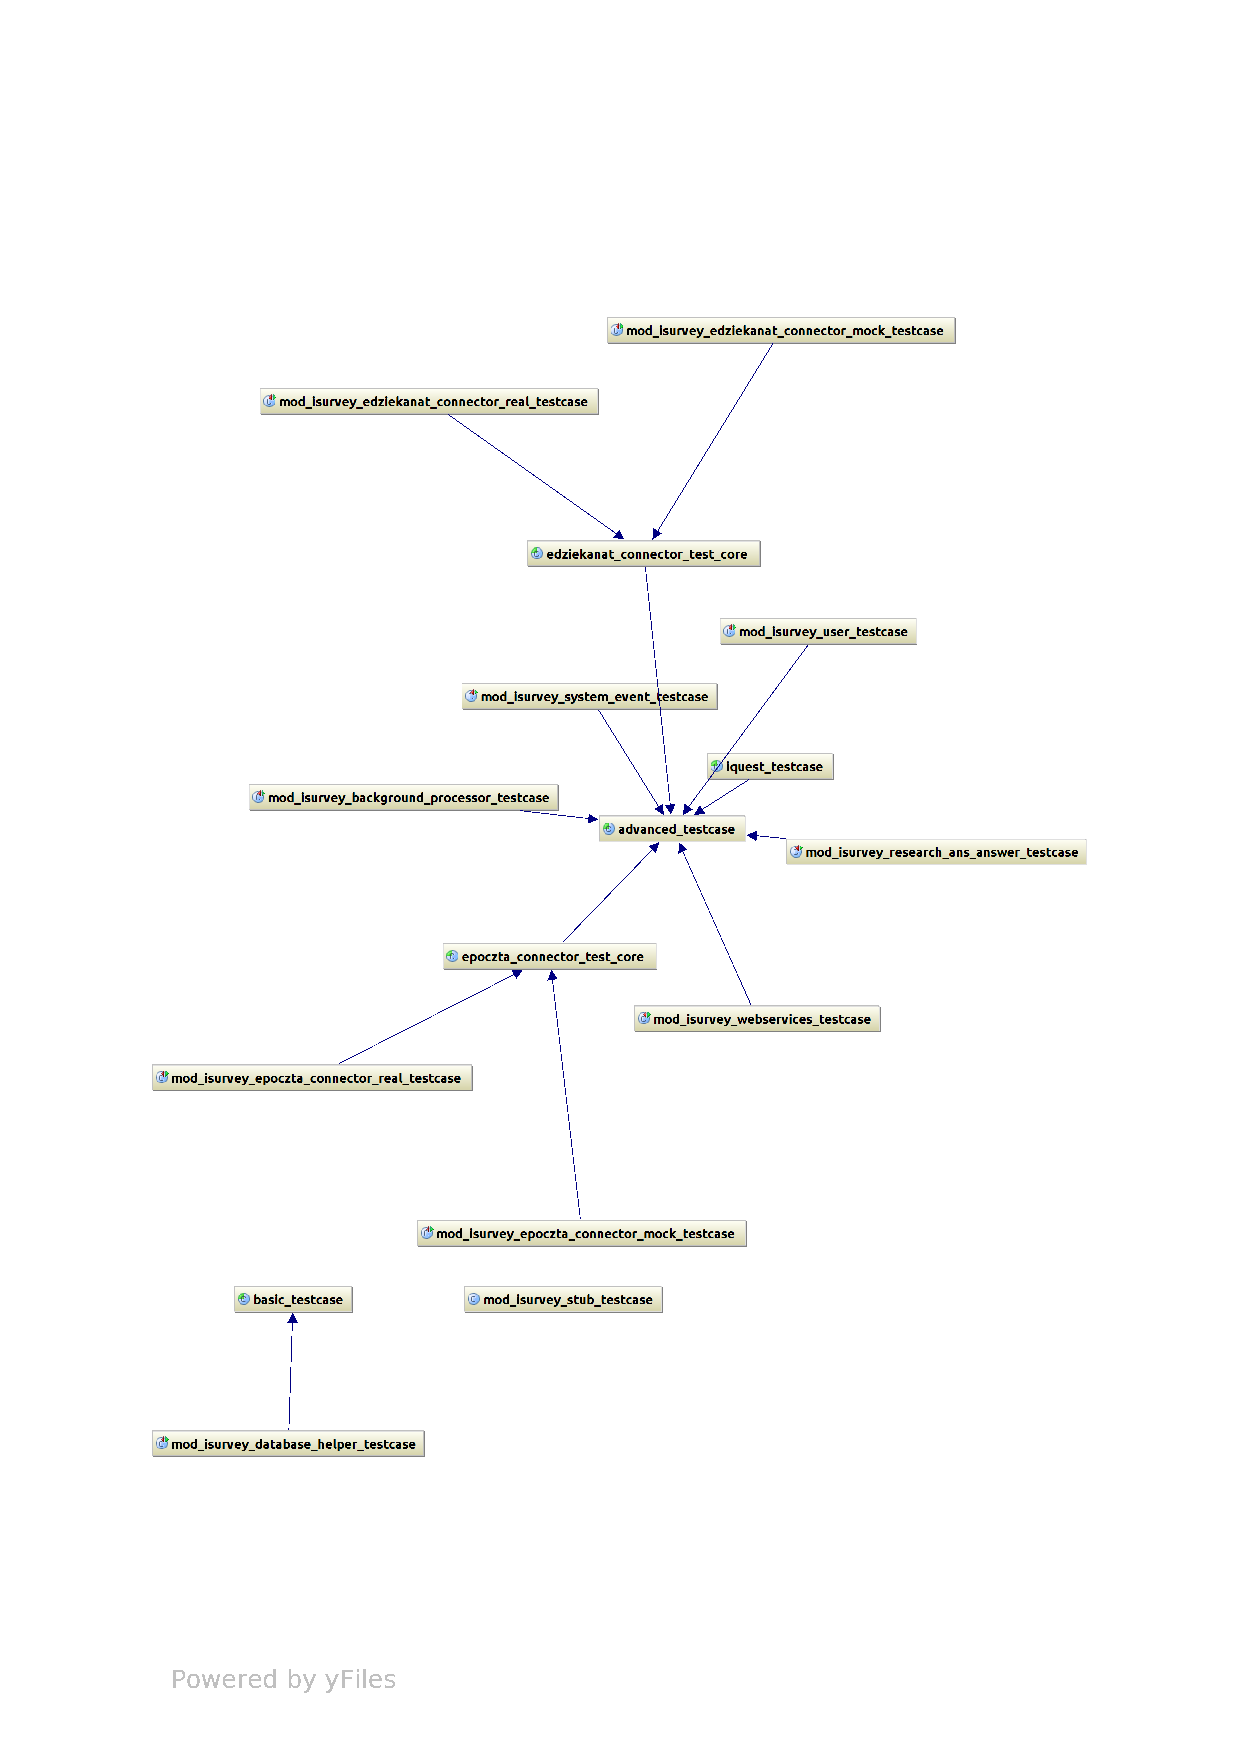
\includepdf{figures/lw/tests1.pdf} 
\end{center}
\caption{Struktura klas testujących (1) (wyk. Łukasz Wieczorek)}\label{fig:tests1}
\end{figure}
\newpage
\begin{figure}[H]
\begin{center}
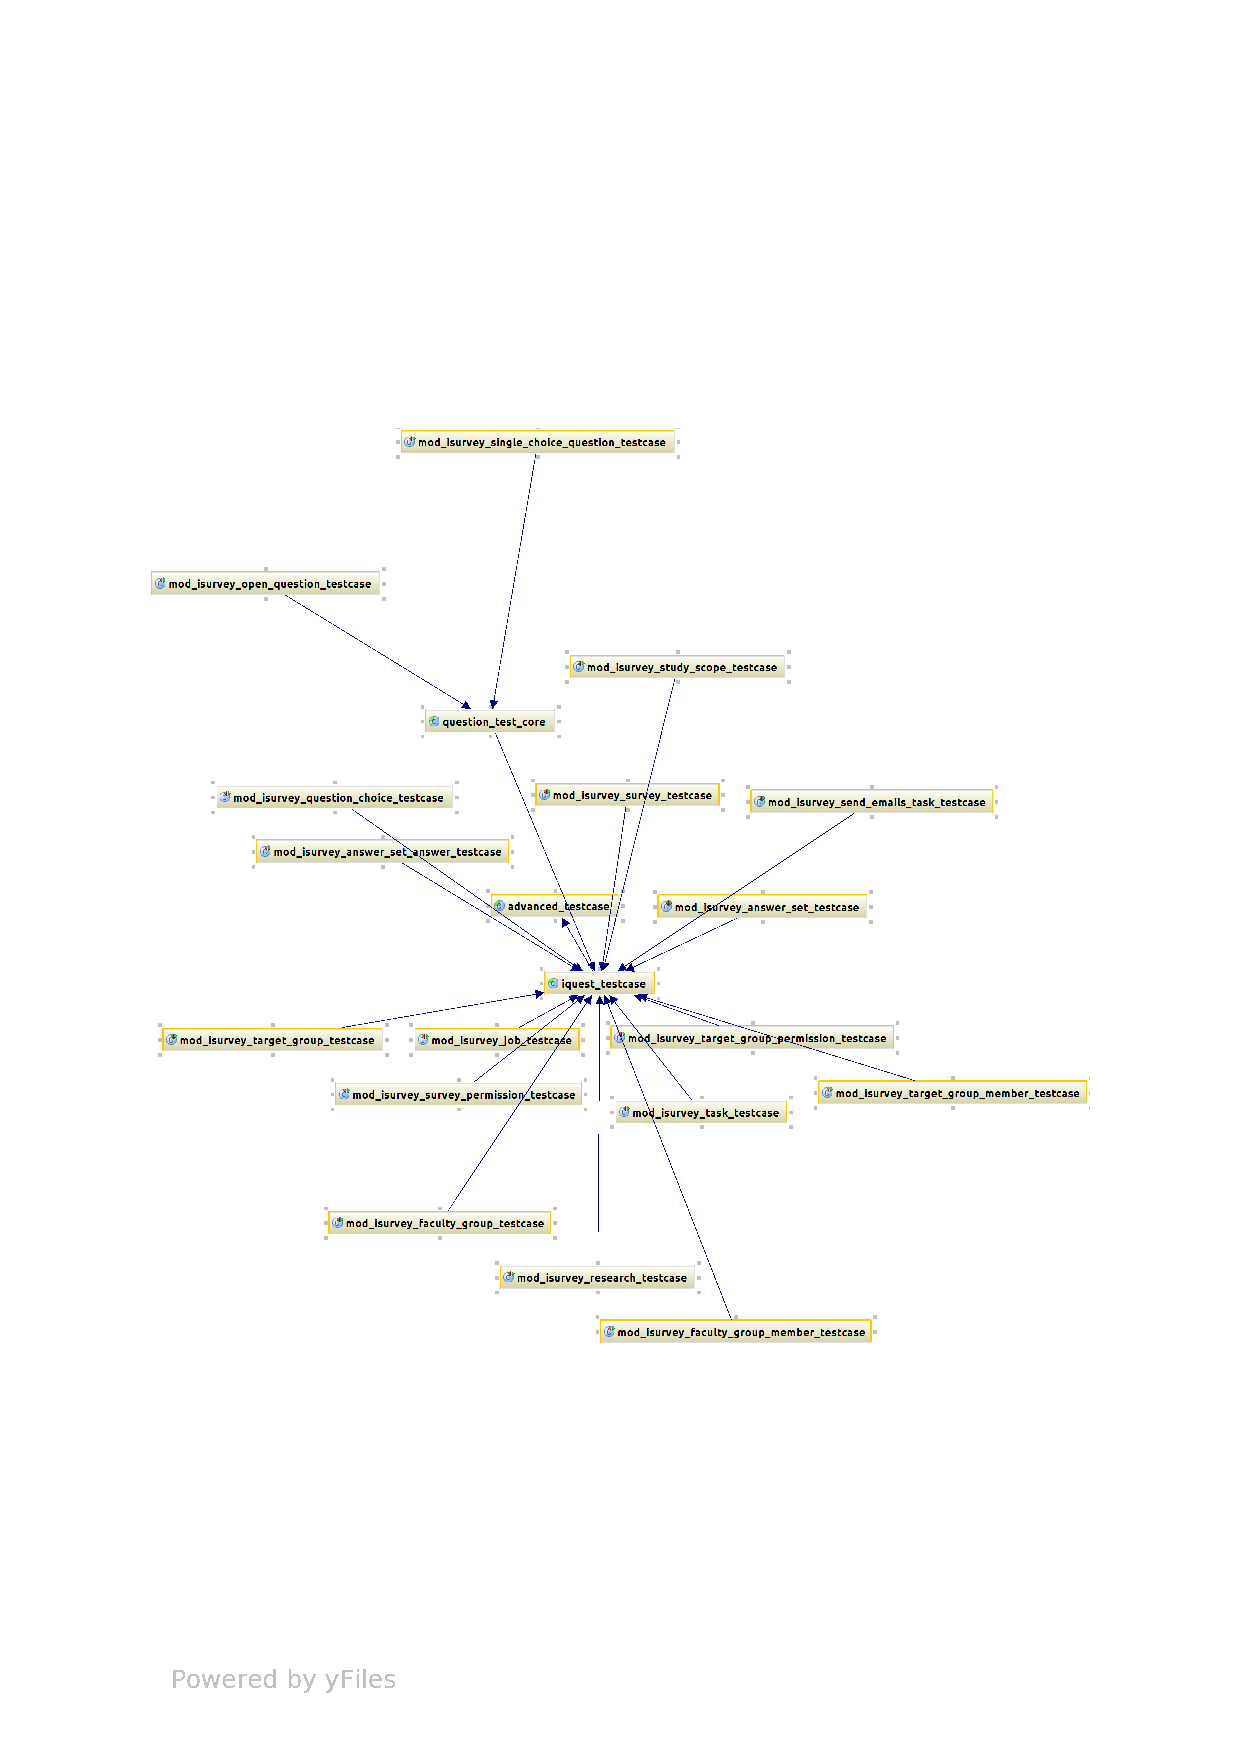
\includegraphics[width=\textwidth]{figures/lw/tests2.pdf} 
\end{center}
\caption{Struktura klas testujących (2) (wyk. Łukasz Wieczorek)}\label{fig:tests2}
\end{figure}
\newpage

Na diagramach widoczne są trzy klasy służące do testowania, z~których dziedziczą wszystkie inne:
\begin{description}
\item[basic\_testcase] -- podstawowe testy jednostkowe
\item[advanced\_testcase] -- testy z użyciem bazy danych
\item[iquest\_testcase] -- rozszerzenie \textit{advanced\_testcase} na potrzeby testowania klas dziedziczących z \emph{record}
\end{description}

\section{Testy akceptacyjne}
\label{Chapter73}

Na początku projektu, przygotowano program w~języku \textit{Java}, uruchamiający zestaw testów akceptacyjnych. W~drugim wydaniu korzystano jednak wyłącznie z~\textit{Selenium IDE}, ze~względu na~możliwość szybszego rozpoznania problemów z~poziomu przeglądarki, w~przeciwieństwie do~terminala.

Testy akceptacyjne rozpatrywane są na dwóch poziomach: automatycznym i~manualnym. Różnica polega jedynie na~tym, kto~(lub~co) wykonuje test - komputer z~odpowiednim oprogramowaniem, czy~człowiek.

\subsection{MAT}
\label{Chapter731}
Poniżej przedstawiono wybrane Manualne Testy Akceptacyjne:

\matbegin{TC1}{Logowanie do systemu przez \textit{eKonto}}
\matpres
\matpre{Użytkownik jest niezalogowany}
\matpre{Użytkownik posiada \textit{eKonto}}
\matpre{Połączenie z Internetem}
\matsteps
\matstep{1}{Użytkownik wybiera opcję ,,zaloguj się''}{Strona logowania do system \textit{iQuest}}
\matstep{2}{Użytkownik naciska przycisk ,,Zaloguj przez eKonto''}{Strona logowania \textit{eLogin}}
\matstep{3}{Użytkownik wpisuje dane logowania}{}
\matstep{4}{Użytkownik naciska przycisk ,,Zaloguj''}{Przekierowanie na stronę systemu \textit{iQuest}, wyświetlenie strony głównej z zalogowanym użytkownikiem.}
\matremark{}

\matbegin{TC2}{Stworzenie Ankiety}
\matpres
\matpre{Zalogowany użytkownik z prawem do tworzenia ankiet}
\matpre{Użytkownik w trakcie przeglądania swojego katalogu ankiet}
\matsteps
\matstep{1}{Użytkownik wybiera przycisk ,,Stwórz ankietę''}{Strona umożliwiająca tworzenie ankiet}
\matstep{2}{Użytkownik podaje nazwę ankiety}{}
\matstep{3}{Użytkownik podaje wstęp i podsumowanie ankiety}{}
\matstep{4}{Użytkownik wybiera opcję definiowania pytań}{Interfejs dodawania pytań}
\matstep{5}{Użytkownik dodaje pytanie jednokrotnego wyboru}{Pojawia się pole na wpisanie treści pytania}
\matstep{6}{Użytkownik wpisuje treść pytania}{}
\matstep{7}{Użytkownik naciska przycisk ,,Dodaj odpowiedź'' dwukrotnie}{Pojawiają się dwa pola do wpisania możliwych odpowiedzi}
\matstep{8}{Użytkownik podaje treści możliwych odpowiedzi}{}
\matstep{9}{Użytkownik dodaje stronę wciskając przycisk ,,Dodaj stronę''}{Wyświetla się nowa strona na dodawanie pytań}
\matstep{10}{Użytkownik dodaje pytanie otwarte}{Wyświetla się pole na wpisanie treści pytania}
\matstep{11}{Użytkownik wpisuje treść pytania}{}
\matstep{12}{Użytkownik wybiera przycisk ,,Zapisz zmiany''}{Komunikat o pomyślnym stworzeniu ankiety}
\matremark{}

\begin{table}[H]
\centering
\begin{tabular}{ | >{\bfseries}c | p{5cm} | } \hline
Krok & \textbf{Dane} \\ \hline
2 & ,,Ankieta testowa'' \\ \hline
3 & ,,Wstęp'' oraz ,,Podsumowanie'' \\ \hline
5 & ,,Pytania jednokrotnego wyboru działają?'' \\ \hline
7 & ,,tak'' oraz ,,nie'' \\ \hline
10 & ,,Pytania otwarte działają?'' \\ \hline
\end{tabular}
\caption{Poprawne dane dla scenariusza TC2}\label{tab:TC2-correct}
\end{table}

\matbegin{TC2.2}{Stworzenie Ankiety - brak pytań}
\matpres
\matpre{Zalogowany użytkownik z prawem do tworzenia ankiet}
\matpre{Użytkownik w trakcie przeglądania swojego katalogu ankiet}
\matsteps
\matstep{1}{Użytkownik wybiera przycisk ,,Stwórz ankietę''}{Strona umożliwiająca tworzenie ankiet}
\matstep{2}{Użytkownik podaje nazwę ankiety}{}
\matstep{3}{Użytkownik podaje wstęp i podsumowanie ankiety}{}
\matstep{4}{Użytkownik wybiera przycisk ,,Zapisz zmiany''}{Komunikat o braku pytań w ankiecie}
\matremark{}

\matbegin{TC3}{Edycja ankiety}
\matpres
\matpre{Zalogowany użytkownik z prawem do tworzenia ankiet}
\matpre{Użytkownik posiada prawo do edycji ankiety ,,Ankieta testowa''}
\matpre{Użytkownik w trakcie przeglądania swojego katalogu ankiet}
\matsteps
\matstep{1}{Użytkownik wybiera przycisk ,,edytuj'' przy „Ankiecie Testowej''}{Strona umożliwiająca edycję „Ankiety Testowej''}
\matstep{2}{Użytkownik wciska przycisk ,,usuń'' przy pytaniu drugim}{Pytanie drugie znika}
\matstep{3}{Użytkownik naciska przycisk ,,Dodaj odpowiedź'' przy pytaniu pierwszym}{Pojawia się pole do wpisania możliwej odpowiedzi}
\matstep{4}{Użytkownik wpisuje możliwą odpowiedź}{}
\matstep{5}{Użytkownik wybiera przycisk ,,Zapisz zmiany''}{Strona wyświetla komunikat potwierdzający zapisanie zmian w ankiecie.}
\matremark{Edytowane mogą być jedynie ankiety, na które nie udzielono jeszcze żadnej odpowiedzi}

\begin{table}[H]
\centering
\begin{tabular}{ | >{\bfseries}c | p{5cm} | } \hline
Krok & \textbf{Dane} \\ \hline
5 & ,,nie wiem'' \\ \hline
\end{tabular}
\caption{Poprawne dane dla scenariusza TC3}\label{tab:TC3-correct}
\end{table}

\matbegin{TC3}{Edycja ankiety - usunięcie wszystkich pytań}
\matpres
\matpre{Zalogowany użytkownik z prawem do tworzenia ankiet}
\matpre{Użytkownik posiada prawo do edycji ankiety ,,Ankiety testowej''}
\matpre{Użytkownik w trakcie przeglądania swojego katalogu ankiet}
\matsteps
\matstep{1}{Użytkownik wybiera przycisk ,,edytuj'' przy „Ankiecie Testowej''}{Strona umożliwiająca edycję ,,Ankiety Testowej''}
\matstep{2}{Użytkownik wciska przycisk ,,usuń'' przy każdym z pytań}{Pytania znikają}
\matstep{3}{Użytkownik wybiera przycisk ,,Zapisz zmiany''}{Strona wyświetla komunikat, że ankieta nie posiada pytań i prosi o ich dodanie.}
\matremark{Edytowane mogą być jedynie ankiety, na które nie udzielono jeszcze żadnej odpowiedzi}

\matbegin{TC4}{Wybranie grupy docelowej}
\matpres
\matpre{Zalogowany użytkownik z prawami do tworzenia ankiet}
\matpre{Użytkownik posiada prawa do ankiety ,,Ankieta Testowa'' oraz badania ,,Badanie Testowe''}
\matpre{Użytkownik posiada prawo do ankietowania grupy docelowej ,,test''}
\matsteps
\matstep{1}{Użytkownik wybiera przycisk ,,Włącz tryb edycji''}{Interfejs edycji \textit{Moodle}}
\matstep{2}{Użytkownik wybiera przycisk „edytuj'' przy ,,Badaniu Testowym''}{Strona umożliwiająca edycję ,,Ankiety Testowej''}
\matstep{3}{Użytkownik wybiera grupę docelową ,,test''}{}
\matstep{4}{Użytkownik wybiera przycisk ,,Zapisz zmiany''}{Strona wyświetla komunikat, że ankieta została zaktualizowana pomyślnie.}
\matstep{5}{Respondent otrzymuje e-mail z powiadomieniem o ankiecie}{}
\matremark{}

\matbegin{TC5}{Udzielanie odpowiedzi}
\matpres
\matpre{Zalogowany użytkownik}
\matpre{Użytkownik znajduje się w grupie docelowej ankiety ,,testowa''}
\matpre{Użytkownik nie odpowiadał udzielał odpowiedzi na ankietę ,,testowa''}
\matsteps
\matstep{1}{System prezentuje ankiety na które użytkownik jeszcze nie odpowiedział}{}
\matstep{2}{Użytkownik wybiera ankietę ,,testowa''}{System prezentuje ankietę}
\matstep{3}{Użytkownik zaznacza odpowiedź na pytanie 1 jako ,,tak''}{}
\matstep{4}{Użytkownik podaje odpowiedź na pytanie drugie jako ,,tak''}{}
\matstep{5}{Użytkownik potwierdza wypełnienie ankiety przyciskiem ,,Wyślij''}{System prezentuje ankiety na które użytkownik jeszcze nie odpowiedział oraz komunikat o pomyślnym przesłaniu odpowiedzi}
\matstep{6}{Respondent otrzymuje e-mail z powiadomieniem o ankiecie}{}
\matremark{}

\matbegin{TC6}{Sprawdzenie wyników}
\matpres
\matpre{Zalogowany użytkownik z prawem do oglądania wyników ankiety ,,Testowa''}
\matsteps
\matstep{1}{Użytkownik wybiera badanie, którego podstawowe wyniki chce sprawdzić}{System prezentuje podsumowanie ankiety \textit{Moodle}}
\matremark{Dotyczy podstawowych wyników. Wyniki zaawansowane obsługuje zewnętrzny serwer \textit{BI}}

\matbegin{TC7}{Dodawanie grupy docelowej}
\matpres
\matpre{Zalogowany administrator z prawami do tworzenia grup docelowych}
\matpre{Brak w systemie grupy docelowej ,,Grupa 1''}
\matsteps
\matstep{1}{Administrator wybiera przycisk ,,Zarządzaj grupami docelowymi''}{System prezentuje dostępne grupy docelowe w systemie}
\matstep{2}{Administrator wybiera przycisk ,,dodaj''}{System prezentuje interfejs dodawania grupy docelowej}
\matstep{3}{Administrator podaję nazwę nowej grupy ,,Grupa 1” i wskazuje jej członków}{}
\matstep{4}{Administrator wybiera grupę nadrzędną dla nowej grupy docelowej}{System automatycznie zapisują zmiany}
\matremark{Test przygotowany na podstawie makiety systemu \textit{iQuest}}

\matbegin{TC8}{Edycja grupy docelowej}
\matpres
\matpre{Zalogowany administrator z prawami do tworzenia grup docelowych}
\matpre{Grupa docelowa ,,Grupa 1'' istnieje w systemie}
\matsteps
\matstep{1}{Administrator wybiera przycisk ,,Zarządzaj grupami docelowymi''}{System prezentuje dostępne grupy docelowe w systemie}
\matstep{2}{Administrator wybiera przycisk ,,zmień nazwę''}{System prezentuje interfejs zmiany nazwy grupy docelowej}
\matstep{3}{Administrator pozostawia nazwę niezmienioną i zatwierdza zmiany}{System prezentuje dostępne grupy docelowe w systemie}
\matstep{4}{Administrator wybiera grupę nadrzędną dla grupy docelowej i dodaje nowego członka do grupy}{System automatycznie zapisują zmiany}
\matremark{Test przygotowany na podstawie makiety systemu \textit{iQuest}}

\matbegin{TC9}{Logowanie bez użycia \textit{eKonta}}
\matpres
\matpre{Użytkownik jest niezalogowany}
\matpre{Istnieje konto użytkownika w systemie}
\matsteps
\matstep{1}{Użytkownik wpisuje adres systemu}{Strona główna \textit{Moodle} z kursem zawierającym system \textit{iQuest}}
\matstep{2}{Użytkownik naciska przycisk ,,Zaloguj się''}{Strona logowania}
\matstep{3}{Użytkownik wpisuje dane logowania}{}
\matstep{4}{Użytkownik naciska przycisk ,,Zaloguj się''}{Przekierowanie na główną stronę \textit{Moodle} z kursem zawierającym system \textit{iQuest}. Wyświetla się napis: ,,Jesteś zalogowany(a) jako...''}
\matremark{}

Dodatkowo, poniżej znajduje się wykaz mapujący przypadki testowe do przypadków użycia:
\begin{itemize}
\item{TC1.X – UC09 Logowanie do systemu.}
\item{TC2.X – UC01 Stworzenie ankiety}
\item{TC3.X – UC02 Edycja ankiety}
\item{TC4.X – UC03 UC04 Wybranie grupy docelowej, uruchomienie ankiety}
\item{TC5.X – UC05 Udzielenie odpowiedzi}
\item{TC6.X – UC06 Sprawdzenie wyników}
\item{TC7.X – UC07 Tworzenie grupy docelowej}
\item{TC8.X – UC08 Edycja grupy docelowej}
\item{TC9.X – UC09 Logowanie do systemu}
\end{itemize}

\subsection{AAT}
\label{Chapter732}

Automatyczne testy akceptacyjne realizowano w~zgodzie z~testami manualnymi, operując na~tych samych wytycznych. Nagrywanie testów odbywało~się za~pomocą oprogramowania \textit{Selenium IDE}, udostępnianego w~formie rozszerzenia dla~przeglądarki \textit{Mozilla Firefox}. Pierwotnie, testy były konwertowane do~języka \textit{Java}, w~celu uruchamiania ich za~pomocą jego środowiska, oferującego sporą swobodę przy~projektowaniu warunków początkowych i~końcowych dla~testów. Problemy, jakie wynikały z~takiego działania, opisane zostały w~rozdziale~\ref{Chapter6}. Na~ich~podstawie zdecydowano o~pozostaniu w~obrębie \textit{Selenium IDE}, które~samo w~sobie również umożliwia automatyzację. Dla dodatkowego ułatwienia zadania, przygotowano skrypt ustawiający bazę danych w~stan początkowy dla~realizacji testów.

\section{Inne metody zapewniania jakości}
\label{Chapter74}

Konieczność zapewnienia jak najwyższej jakości oprogramowania, wymusiła testowanie w~kontrolowanych warunkach na~różnych urządzeniach. Co~prawda, lokalne serwery developerskie pracowały zawsze w~oparciu o~system \textit{Ubuntu 12.04 LTS}\footnote{\cite{Man:Ubuntu}}, z~serwerem \textit{Apache} i~systemem zarządzania bazą danych \textit{PostgreSQL}, jednak maszyny klienckie były już~znacznie bardziej różnorodne. \\

Testy klienckie odbyły się na komputerach stacjonarnych klasy PC oraz~równoważnych laptopach, z~użyciem zarówno systemów rodziny \textit{Windows} (wersje od~\textit{XP} do~\textit{Win8}), jak~i~\textit{Linux} (wspomniana wcześniej wersja \textit{Ubuntu}) oraz~\textit{Mac~OS~X}. Ponadto, przetestowano trzy główne platformy mobilne (Android, iOS @ iPhone~4S, WP7.x @ Nokia~Lumia~710) poprzez dostęp do~systemu z~poziomu telefonów komórkowych. Komputery użyte do~testów charakteryzowały~się posiadaniem co~najmniej jednordzeniowego procesora ze~zbiorem 32-bitowych~instrukcji i~taktowaniem zegara nie~mniejszym niż~1,5~GHz, oraz~4~GB pamięci~RAM. \\

Na podstawie testów, utworzono dwa raporty: ,,wygląd i~działanie systemu \textit{iQuest} na~platformach mobilnych'' oraz ,,wygląd i~działanie systemu \textit{iQuest} w~różnych konfiguracjach system-przeglądarka'', udostępnione w~ramach systemu zarządzania projektem\footnote{\cite{Redmine:ProjDocs}}. Wynika z~nich, że~system \textit{iQuest} jest~przenośny.